\begin{frame}
  \frametitle{Motivation for MSR Multiphysics Modeling V\&V}
  \begin{columns}
    \column{5.5cm}
      \textbf{Three important multiphysics phenomena in MSRs}
      \begin{itemize}
        \item Salt flow-induced temperature and delayed neutron precursor (DNP) drift
        \item Temperature reactivity feedback due to Doppler broadening and thermal expansion
        \item Buoyancy-driven flow due to temperature gradients
      \end{itemize}
    \column{5.5cm}
      \begin{figure}
        \centering
        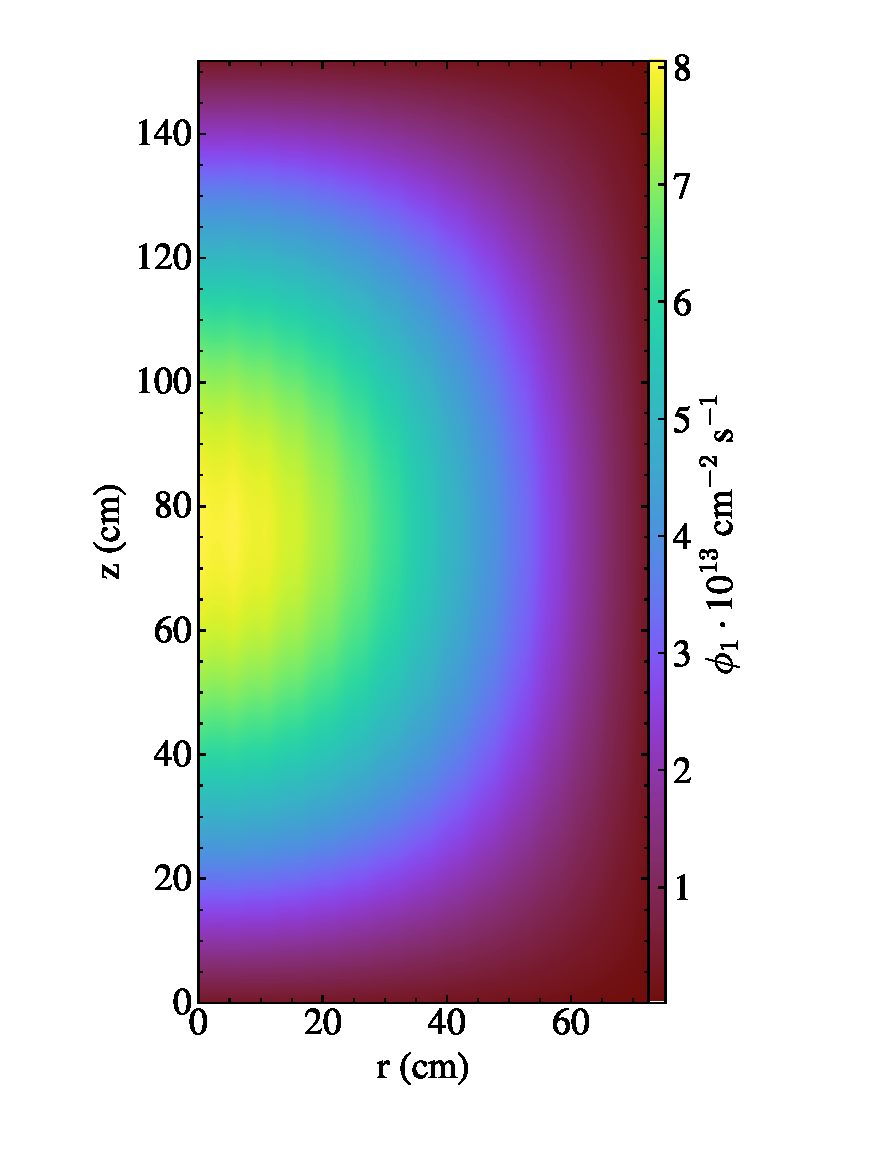
\includegraphics[width=.48\columnwidth]{../images/2d_gamma_heating_group1}
        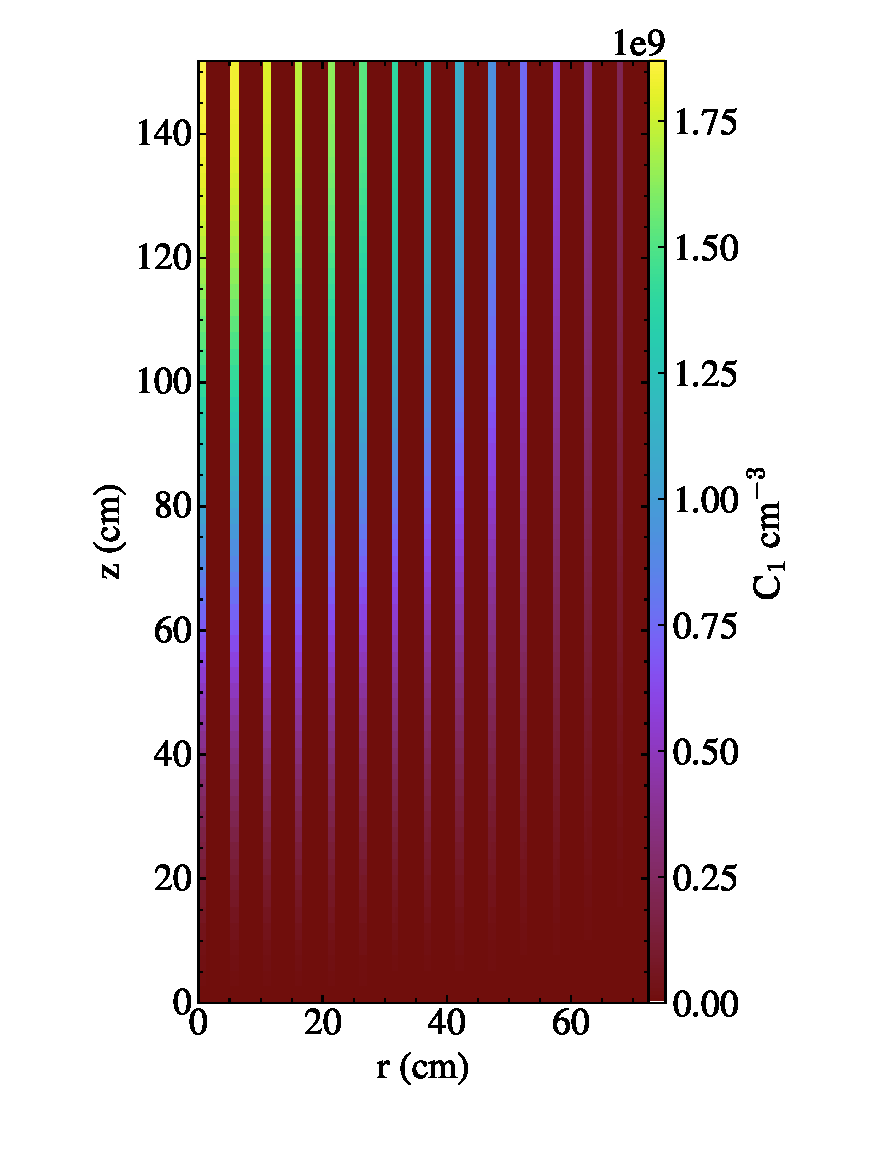
\includegraphics[width=.48\columnwidth]{images/2d_gamma_heating_pre1_scaled}
        \caption{Group 1 neutron flux (left) and the longest-lived precursor group (right) in a 2-D
        MSRE model with upward flow \cite{lindsay_introduction_2018}.}
      \end{figure}
  \end{columns}
\end{frame}

